\documentclass[a4paper]{article}

\usepackage[margin=2cm]{geometry}
\usepackage{fontspec}			% utf-8 suport
\usepackage{amsmath}			% Math utilities
\usepackage{amssymb}			% Math symbols
\usepackage{amsfonts}			% More math fonts
\usepackage{mathtools}			% More math tools (rcases)
\usepackage[makeroom]{cancel}	% Math cancel
\usepackage[catalan]{babel} 	% Language 
\usepackage{listings}			% Code inserting
\usepackage[dvipsnames]{xcolor}	% Color definitions
\usepackage{enumitem}
\usepackage{graphicx}

\setlength{\parindent}{0pt}
\setlength{\parskip}{0.2cm}

\lstset{ % Donat que el paquest listings no té la sintaxi per R definida la hem de definir nosaltres
	language=R,                     % the language of the code
	basicstyle=\ttfamily\footnotesize,       % the size of the fonts that are used for the code
	numbers=left,                   % where to put the line-numbers
	numberstyle=\tiny\color{gray},  % the style that is used for the line-numbers
	stepnumber=1,                   % the step between two line-numbers. If it's 1, each line
	% will be numbered
	numbersep=5pt,                  % how far the line-numbers are from the code
	backgroundcolor=\color{white},  % choose the background color. You must add \usepackage{color}
	showspaces=false,               % show spaces adding particular underscores
	showstringspaces=false,         % underline spaces within strings
	showtabs=false,                 % show tabs within strings adding particular underscores
	frame=single,                   % adds a frame around the code
	rulecolor=\color{black},        % if not set, the frame-color may be changed on line-breaks within not-black text (e.g. commens (green here))
	tabsize=2,                      % sets default tabsize to 2 spaces
	captionpos=b,                   % sets the caption-position to bottom
	breaklines=true,                % sets automatic line breaking
	breakatwhitespace=false,        % sets if automatic breaks should only happen at whitespace
	title=\lstname,                 % show the filename of files included with \lstinputlisting;
	% also try caption instead of title
	keywordstyle=\color{blue},      % keyword style
	commentstyle=\color{OliveGreen},   % comment style
	stringstyle=\color{purple},      % string literal style
	escapeinside={\%*}{*)},         % if you want to add a comment within your code
	morekeywords={*,...}            % if you want to add more keywords to the set
} 


\title{\textsc{APA Problemes} \\ Problema 3 Anàlisi discriminant d'en Fisher en acció}
\author{Lluc Bové \and Raúl Ibáñez \and Joan Marcè \and Aleix Trassera}
\date{}

\begin{document}
\maketitle

\textbf{Considerem un problema amb dades bidimensionals i dues classes:}

\begin{align*}
	C_1 &= \{(4, 1), (2, 4), (2, 3), (3, 6), (4, 4)\} \\
	C_2 &= \{(9, 10), (6, 8), (9, 5), (8, 7), (10, 8)\}
\end{align*}

\begin{enumerate}[resume=main]
	\item \textbf{Calcules les dues mitjanes de classe $m_1$ i $m_2$}
\end{enumerate}
A partir de la definició de $\vec{m}_1$ i $\vec{m}_2$ obtenim:
\begin{align*}
\vec{m}_1 &:= \frac{1}{|C_1|} \sum_{n \in C_1} \vec{x}_n =
\frac{1}{5}
\begin{pmatrix}
15 \\
18
\end{pmatrix}
\\
\vec{m}_2 &:= \frac{1}{|C_2|} \sum_{n \in C_2} \vec{x}_n =
\frac{1}{5}
\begin{pmatrix}
42 \\
38
\end{pmatrix}
\end{align*}

\begin{enumerate}[resume=main]
	\item \textbf{Calculeu les dues matrius de dispersió (\emph{scatter}) intra-classe $S_1$ i $S_2$ i la matriu de dispersió intra-classes total $S_W = S_1 + S_2$.}
\end{enumerate}
Partint també de la definició de $S_1$, $S_2$ i $S_W$ obtenim les matrius de dispersió.
\begin{align*}
	S_1 &= \sum_{n \in C_1} (x_n - \vec{m}_1)(x_n - \vec{m}_1)^T = 
	\begin{pmatrix}
	4 & -2 \\
	-2 & 13,2
	\end{pmatrix} \\
	S_2 &= \sum_{n \in C_2} (x_n - \vec{m}_2)(x_n - \vec{m}_2)^T = 
	\begin{pmatrix}
	9,2 & -0,2 \\
	0,2 & 13,2
	\end{pmatrix}
\end{align*}
$$
S_W = S_1 + S_2 = 
\sum_{n \in C_1} (x_n - \vec{m}_1)(x_n - \vec{m}_1)^T + 
\sum_{n \in C_2} (x_n - \vec{m}_2)(x_n - \vec{m}_2)^T =
\begin{pmatrix}
13,2 & -2,2 \\
-2,2 & 26,4
\end{pmatrix}
$$

\begin{enumerate}[resume=main]
	\item \textbf{Calculeu la matriu de dispersió inter-classes $S_B$.}
\end{enumerate}
$$
S_B = (\vec{m}_2 - \vec{m}_1)(\vec{m}_2 - \vec{m}_1)^T = 
\begin{pmatrix}
29,16 & 21,6 \\
21,6 & 16
\end{pmatrix}
$$

\begin{enumerate}[resume=main]
	\item \textbf{Trobeu la direcció de projecció òptima $w^*$ de dues maneres:}
\end{enumerate}

\begin{enumerate}[resume=second,label=(\alph*),itemindent=1em]
	\item \textbf{Directament amb la fórmula $w^* = S_W^{-1} (m_1 - m_2)$}
\end{enumerate}

$$
w^* = 
\begin{pmatrix}
0,0768 & 0,0064 \\
0,0064 & 0,03841
\end{pmatrix} ·
\begin{pmatrix}
-5,4 \\ -4
\end{pmatrix} =
\begin{pmatrix}
-0,44 \\
-0,19
\end{pmatrix}
$$

\begin{enumerate}[resume=second,label=(\alph*),itemindent=1em]
	\item \textbf{Resolent el problema de vectors propis $(S_W^{-1}S_B)w = \lambda w$.}
\end{enumerate}

$$
w^* = 
\begin{pmatrix}
0,9195 \\
 0,3929
\end{pmatrix}
$$

Es pot comprovar que el vector té la mateixa direcció que el  de l'apartat anterior ja que són linealment dependents.

\begin{enumerate}[resume=main]
	\item \textbf{Representeu gràficament el resultat: dibuixeu les dades, la direcció de projecció òptima $w^*$ i la projecció de les dades}
\end{enumerate}

El gràfic representa cada una de les classes amb els colors verd i vermell respectivament, la recta representa gràficament la direcció $w^*$

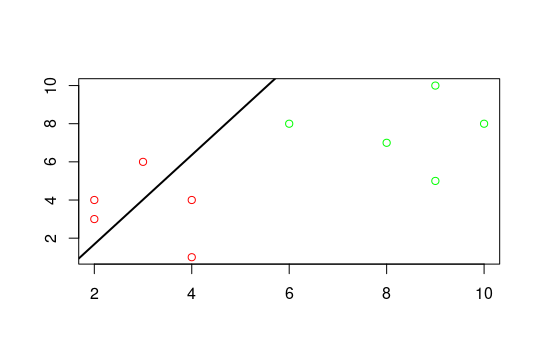
\includegraphics[scale=0.5]{plot}\centering

\end{document}
